\documentclass[12pt, letterpaper]{article}
%, titlepage
\usepackage[left=1in, right=1in]{geometry}                % See geometry.pdf to learn the layout options. There are lots.
%\geometry{letterpaper}                   % ... or a4paper or a5paper or ...
%\geometry{landscape}                % Activate for for rotated page geometry
%\usepackage[parfill]{parskip}    % Activate to begin paragraphs with an empty line rather than an indent
\usepackage{graphicx, subfigure}
\usepackage{amssymb}
\usepackage{epstopdf}
\usepackage{amsmath}
\usepackage{setspace}
\usepackage{amsthm}
\usepackage{natbib}
\usepackage{booktabs}
\usepackage{rotating}
\usepackage{multirow}
\usepackage{pbox}
\usepackage{url}
\newtheorem{hyp}{Hypothesis} 
\usepackage{appendix}
% \usepackage[nolists, nomarkers, heads]{endfloat}
\setcounter{secnumdepth}{2}
\usepackage[T1]{fontenc}
%\usepackage{fourier}

\def\citepos#1{\citeauthor{#1}'s (\citeyear{#1})} % possessive citations


\DeclareGraphicsRule{.tif}{png}{.png}{`convert #1 `dirname #1`/`basename #1 .tif`.png}


\author{Andrew W. Pierce \\ University of Georgia \and Steven W. Webster \\ Washington University in St. Louis}
\title{How Race Influences the Impact of Anger on Trust in Government}
\date{\today}

%\usepackage{Sweave}
\begin{document}
%\Sconcordance{concordance:anger_trust_manuscript.tex:anger_trust_manuscript.Rnw:%
1 7 1 1 0 8 1}


\begin{titlepage}
\maketitle

\thispagestyle{empty}

\begin{singlespacing}
\abstract{whatever}
\end{singlespacing}

\end{titlepage}

%%%%%%%%%%
% end title page %
%%%%%%%%%%

\newpage
\setcounter{page}{1}

\doublespacing

\section{Empirical Estimation}
\label{sec:design}

\subsection{Observational Analysis}
\label{subsec:anes}

To examine how racial identity conditions the relationship between anger and trust in government, we first begin by utilizing data from the 2016 American National Election Studies (ANES). The ANES is useful for our purposes because, in addition to its large sample size, it contains the three variables essential to this analysis: a measure of trust in government, measures of anger, and information about each respondent's racial identity.

Though there are many possible ways to measure trust in government, here we are focused on one specific aspect of governmental trust: respondents' perceptions of whether public officials care about what people think. This measure is captured by asking individuals to rate their level of agreement with the following statement: ``public officials don't care what people think." Responses take on five possible values, ranging from ``disagree strongly" to ``agree strongly." We then recode this variable numerically to range from 0-4, where higher values indicate higher levels of \emph{dis}trust in government.

To measure individuals' level of anger, we analyze the frequency with which individuals reported feeling angry at the opposing party's presidential candidate. Thus, for Republican respondents, our measure of anger captures how often he or she felt angry toward Hillary Clinton. Similarly, for Democratic respondents, our measure of anger captures how often he or she felt angry toward Donald Trump. We normalize this variable to range from 0-1, where zero indicates that an individual never felt angry toward the opposing party's candidate and one indicates that an individual reported that they ``always" felt angry toward the opposing party's candidate. 

Finally, to analyze how an individual's racial identity conditions the relationship between anger and his or her level of trust in government, we utilize individuals' responses to the question asking about racial affiliation. Potential responses are White, non-Hispanic; Black, non-Hispanic; Asian, native Hawaiian or other Pacific Islander; Native American; and Hispanic. We then collapse responses to this question into a dummy variable indicating whether an individual identifies as something other than White. Though this obscures any potential differences in the ways in which specific non-White racial identities condition the relationship between anger and trust in government, this approach allows us to establish a baseline as to whether such racial differences exist at all.

To estimate whether racial identity conditions the relationship between anger and trust in government, we employ a series of Bayesian Additive Regression Tree (BART) models. Unlike traditional linear models, BART models do not impose any linearity conditions on the data. Moreover, BART models produce an estimate as to the relationship between anger and trust in government for each individual in our data. Thus, we are able to easily examine potential non-linearities between anger and trust in government, as well as the ways in which racial identities condition this relationship. To reduce confounding in our estimation we also include controls for individuals' self-reported ideology, their gender, their level of education, their degree of political activism, and pre-election levels of trust in government.\footnote{The political activism scale is an additive measure of 11 different campaign-related activities. These activities include attending political meetings; talking to others about politics; wearing a campaign button; working for a political party; contributing money to a party, candidate, or third-party organization; joining a political protest; attending a school board meeting; contacting a Member of Congress; and signing a petition.} The results of the BART model are shown in Figure \ref{fig:bart-results}.

\begin{center}
\begin{figure}
\begin{center}
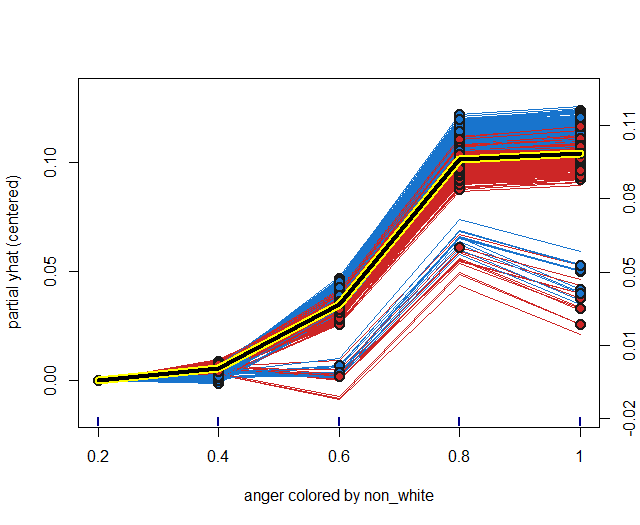
\includegraphics[width=\textwidth]{bart_model}
\caption{\footnotesize\textit{Anger, Race, and Trust in Government.} This figure shows the non-linear relationship between anger and trust in government. It also shows that the relationship between anger and trust in government is stronger for those individuals who identify as non-White.}
\label{fig:bart-results}
\end{center}
\end{figure}
\end{center}

The results of the BART model displayed in Figure \ref{fig:bart-results} reveal two interesting patterns. The first is that the relationship between anger and trust in government is non-linear. As can be seen, there is very little relationship between anger and trust in government at low levels of individual anger. When individuals move into the middle range of anger there appears to be a slightly more detectable relationship between anger and trust in government. However, when individuals become really angry there is a strong connection between anger and levels of trust in government. Indeed, the jump from the median level to the next highest level of anger produces a dramatic increase in the likelihood that an individual distrust the government. This relationship increases slightly more when individuals are at the highest level of anger. Accordingly, these patterns suggest that, though anger is certainly related to distrust in government, this distrust really begins to manifest when individuals are exhibiting high levels of anger.

The second pattern that emerges from the BART model displayed in Figure \ref{fig:bart-results} is that the relationship between anger and trust in government is conditioned by an individual's racial affiliation. In Figure \ref{fig:bart-results}, the relationship between anger and trust in government is shaded in red for Whites and shaded in blue for non-Whites. As can be seen, the relationship between anger and trust in government is stronger for non-Whites at almost every level of anger. Indeed, it is only at the very lowest levels of anger that the relationship between anger and trust in government is stronger for Whites than non-Whites. At every other level of anger, the results of the BART model suggest that anger is more closely related to distrust in government for non-Whites than for Whites.

\subsection{Experimental Design}
\label{subsec:experiment}

The preceding analysis has established that anger is related to trust in government, that this relationship is non-linear, and that the relationship between these two variables is stronger for those who are non-White than for those who are White. However, as the model presented in Figure \ref{fig:bart-results} relies on observational data, it is not possible for us to say from these results that anger causes distrust in government, nor does it allow us to say that the causal effect of anger on governmental distrust is stronger for non-Whites than for Whites.

To explore whether the relationship between anger and trust in government is causal in nature, we employ a survey experiment that exogenously varies individuals' level of anger. The survey experiment was fielded throughout the country in the fall of 2016 via Survey Sampling International (SSI) and was finished a few months before the U.S. presidential election. The experimental data is comprised of 3,262 respondents, all of whom are registered to vote in the United States. 

The data for this study contains a pre- and post-experiment survey. Before the experiment, participants were asked to fill out a series of demographic questions. These questions include the respondent's year of birth, gender, race, yearly income, and and level of education. Participants were also asked a series of political identification questions. These questions include an individual's partisan affiliation and ideological leanings, both of which are measured on a seven-point scale.\footnote{These questions are analogous to those used in typical datasets, such as the American National Election Studies or the Cooperative Congressional Election Study.} Individuals were also asked about their past forms of political participation and level of interest in politics and political affairs.

The experimental manipulation of the study is designed to increase individuals' level of anger. In order to do this, we rely on a technique known as ``emotional recall" \citep{lerneretal2003effects, lerner_kelter2001}. This manipulation asks individuals to write a detailed paragraph about a time they felt a given emotion (here, anger), with the expectation that writing about their experience will cause an individual to temporarily relive the triggered emotion. Such a design has become widespread in political science, and has been most notably used to study the effect of emotions on Americans' views toward terrorism \citep{lerneretal2003effects}, likelihood of participating in politics \citep{vbggh}, and seeking information about politics \citep{valentinoetal2008}.

However, the experimental manipulation used in this study differs from previous uses of the technique in an important way. Typical emotional recall designs ask individuals to recount a time that they felt a particular emotion about politics. By phrasing the experimental prompt in such a way, it is likely that scholars are unintentionally introducing confounding considerations into their designs. Indeed, when the experimental prompt is phrased in such a way, it is impossible to tell whether individuals are reacting to a prompt to exhibit a higher degree of some emotion, or if they are responding to the increased salience of politics or political issues. In order to disentangle this methodological problem and obtain more valid estimates as to the causal effect of anger on rational miscalculations, the experimental recall design that we use separates the emotion (anger) from the target (politics) \citep[see also,][]{webster2017}. Thus, our design randomizes individuals into one of three treatment groups. In the first treatment group, individuals are asked to recall a time they were very angry, and to describe this time in such a way that an individual who was reading the response might also become angry. The second treatment group asks individuals to write about a time they were very angry specifically about politics, while the third treatment group asks individuals to write about a time they thought about politics. This simple modification of the experimental wording allows us to avoid concerns about confounding factors that plague other studies and, as a result, be more certain that the experimental manipulation is altering levels of anger and \emph{not} merely increasing the salience of political issues.

After the experimental manipulation, subjects were asked to rate their level of agreement or disagreement with the following statement: ``The national government is unresponsive to the concerns and interests of the public." Agreement is assessed on a 0-10 scale, where higher scores indicate more agreement. Thus, higher values indicate a greater level of distrust in the national government.

The unconditional expectation is that those individuals who were randomized into one of the two anger-inducing treatment groups should be more distrustful of the national government. In other words, they should give higher ratings on the post-experiment question about the government's responsiveness to the concerns and interests of the public. However, the key focus of this paper is how the relationship between anger and trust in government is moderated by the race of the respondent. As described in Section \ref{sec:theory}, our expectation is that the effect of anger on reducing trust in government should be stronger for non-Whites. Given the randomized nature of the experimental design, estimation occurs via a simple ordinary least squares (OLS) model as shown in Equation \ref{eq:experiment-model}.

\vspace{-13mm}
\begin{center}
\begin{equation}
y_i = \alpha + \beta_1\textrm{Anger} + \beta_2\textrm{PoliticalAnger} + \beta_3\textrm{PoliticalSalience} + \epsilon
\label{eq:experiment-model}
\end{equation}
\end{center}

To test for heterogeneous treatment effects by individuals' racial affiliation, we subset the model shown in Equation \ref{eq:experiment-model} to include only those individuals who racially identify as something other than White. Estimating our model only on the subset of individuals who identify as non-White functionally achieves the same thing as including a series of dummy variables for non-White respondents and interacting them with the indicators for treatment status. However, to facilitate a comparison of the relationship between anger and trust in government for Whites and non-Whites, we also estimate Equation \ref{eq:experiment-model} on the entire sample. We then simultaneously present the results of these two models in Figure \ref{fig:coef_plot}.

The results of our experimental analyses largely corroborate the results of our observational analysis. Indeed, the results of our experimental manipulation suggest that the strength of the relationship between anger and reduced trust in government is dependent upon one's racial affiliation. Recall that the expectation is that those individuals who were randomized into one of the treatment groups that sought to prime anger should be more distrustful of the national government. Mechanically, this implies that the coefficient on the treatment indicators for the anger-only condition and the anger-about-politics condition should be positive. The results, shown in Figure \ref{fig:coef_plot}, provide a considerable amount of support for this hypothesis.

The results indicate that anger has differential effects depending upon whether an individual is White or non-White. Among White participants ($n=2666$), apolitical anger increases distrust in the national government ($p < .05$) as does targeted political anger ($p < .1$). Merely thinking about politics does not have any statistically significant effect on trust in government. The results for non-White participants ($n=586$) are slightly different. Among non-Whites, apolitical anger has no statistically discernible effect on lowering trust in government. However, non-White individuals who were randomized into the targeted political anger condition exhibit a greater amount of distrust in the national government than White individuals who were randomized into this same treatment condition. Moreover, for non-White experiment participants, merely \emph{thinking} about politics served to reduce trust in the national government. Taken together, these results suggest that anger's ability to reduce the citizenry's trust in the national government, and the extent to which it does so, is, to a degree, conditional upon an individual's racial identity.

\begin{center}
\begin{figure}
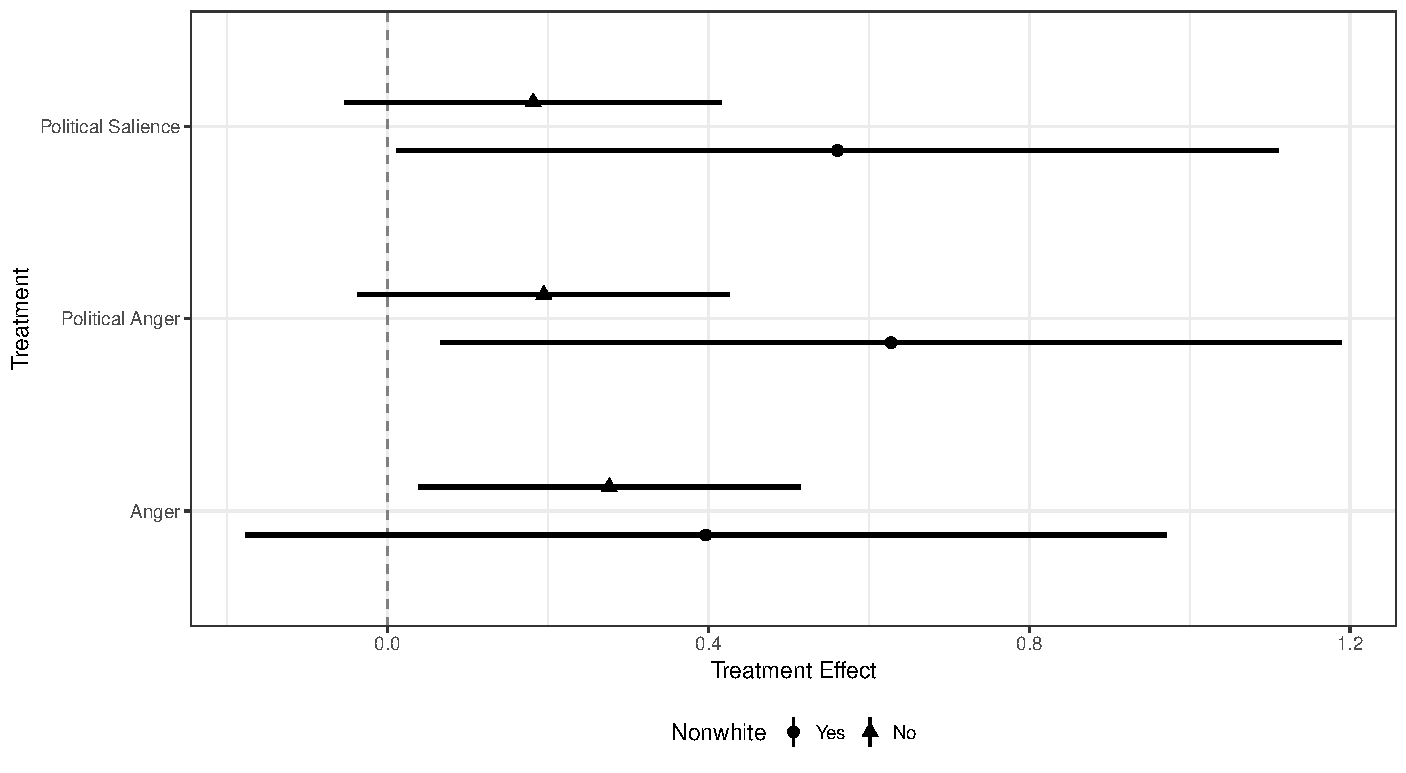
\includegraphics[width=\textwidth]{coefs}
\caption{\footnotesize\textit{The Relationship Between Anger, Race, and Trust in Government.} This figure shows the coefficient estimates from the experimental manipulation that sought to induce anger in participants. The figure suggests that higher levels of anger reduces trust in government and that this effect is greater for non-White individuals.}
\label{fig:coef_plot}
\end{figure}
\end{center}


\newpage
\begin{singlespacing}
\bibliographystyle{apsr.bst}
\bibliography{anger_race_bib}
\end{singlespacing}



\end{document}
